\section{Models against each other and against perfect play}\label{sec:comparisons}

Sections \ref{old:7}--\ref{old:9} compared models through win rates against the two scripted tigers. With the
game solved, three sharper questions can be asked. How do the models fare against each other? How do they
fare against a player that never errs? And, move by move, how often do they change the value of the
position? The experiment is \code{perfect\_play/compare\_models.py}; its results are in
\code{perfect\_play/tables/model\_comparison.json}.

\subsection{Setup}\label{sec:cmp-setup}

\textbf{Players.} Table~\ref{tab:players} lists them. Models play their deterministic masked move
(Section~\ref{old:3.2}), as in all earlier evaluations.

\begin{table}[H]
\centering\small
\caption{Players in the comparison.}\label{tab:players}
\begin{tabular}{@{}>{\raggedright\arraybackslash}p{0.22\linewidth}p{0.74\linewidth}@{}}
\toprule
Name & Player \\
\midrule
Perfect & reads the tables: fastest win, slowest loss. Among drawing moves it prefers positions not yet seen in the game, then the move after which the largest share of the opponent's replies lose (``trap-seeking'') \\
Perfect (plain) & reads the tables; picks uniformly among the moves of equal value and distance, with no preference among drawing moves \\
Random & uniform over legal moves \\
Greedy, Smart & the scripted tigers of Section~\ref{old:2.4} \\
NormalGoat, SmartGoat, RobustGoat & the shipped goat models (Section~\ref{old:6.2}; 100M, 100M and 60M steps) \\
PPO+nll & plain PPO with the legality loss, $c_{\text{legal}} = 0.5$, tanh, seed 42, 10M steps (Section~\ref{old:6.4}) \\
ReLU-Mask & Maskable PPO, ReLU, seed 42, 10M steps (Section~\ref{old:6.4}) \\
Tiger-N, Tiger-S, RobustTiger & the shipped tiger models, trained against NormalGoat, SmartGoat and RobustGoat \\
\bottomrule
\end{tabular}
\end{table}

\textbf{Games.} Every goat player meets every tiger player in 200 games from the opening, goats first, under
\code{TnGEnv}'s limits (200 plies; fourth repeat of a board with the goats to move). Game $i$ uses seed
$20{,}000 + i$ for all random choices. Two models always play the same game, so those pairings have one game.

\textbf{Judging moves.} Before and after each move the exact value of the position is read from the tables.
A move is a \textbf{blunder} if it lowers the value for the side that made it:
$\W{\to}\D$ (a forced win becomes a draw), $\W{\to}\Lo$, or $\D{\to}\Lo$ (a draw becomes a forced loss). All
other moves are value-preserving. A perfect player makes no blunders by construction; the tables confirm it
on its 382{,}163 decisions here.

\subsection{Results}

\begin{table}[H]
\centering\footnotesize
\caption{Round robin. Each cell is \emph{goat wins / tiger wins} in percent of 200 games; the rest are draws
by the turn limit or the repeat rule. $^\dagger$~Two deterministic models play one game: G, T or D is its
result.}\label{tab:roundrobin}
\begin{tabular}{@{}l cccccccc@{}}
\toprule
\tabin{generated/tab_roundrobin_head}
\midrule
\tabin{generated/tab_roundrobin}
\bottomrule
\end{tabular}
\end{table}

\begin{figure}[H]
\centering
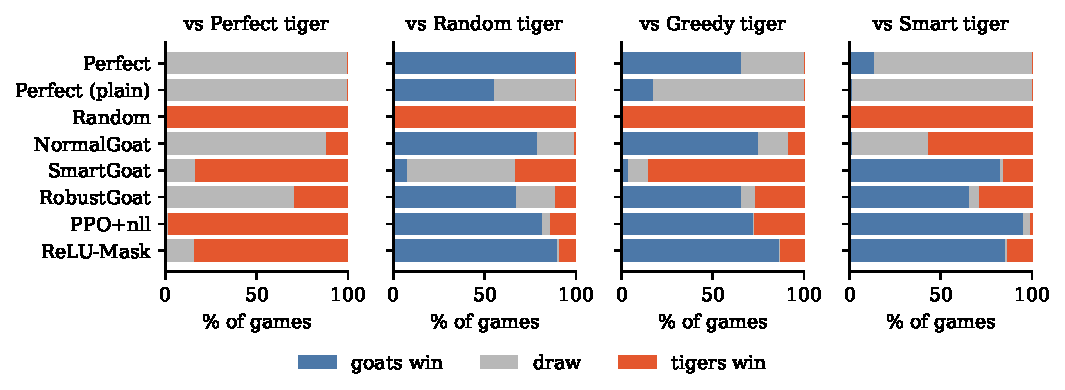
\includegraphics[width=\linewidth]{figures/outcomes_goat_players.pdf}
\caption{Outcomes of each goat player against four reference tigers (200 games each).}\label{fig:outcomes}
\end{figure}

\begin{table}[H]
\centering\footnotesize
\caption{Models against the perfect player, in percent of 200 games. ``Blunders'' is the mean number of
$\D{\to}\Lo$ moves per game; ``first'' is the mean ply of the first blunder in the games that have one.}\label{tab:vsperfect}
\begin{tabular}{@{}ll rrr r rr@{}}
\toprule
\multicolumn{8}{@{}l}{\textbf{Goat players against a perfect tiger}} \\
goats & perfect tiger & wins & draws & losses & plies & blunders & first \\
\midrule
\tabin{generated/tab_goats_vs_perfect}
\midrule
\multicolumn{8}{@{}l}{\textbf{Tiger players against a perfect goat}} \\
tigers & perfect goat & wins & draws & losses & plies & blunders & first \\
\midrule
\tabin{generated/tab_tigers_vs_perfect}
\bottomrule
\end{tabular}
\end{table}

\begin{table}[H]
\centering\footnotesize
\caption{Move quality of each player over all its round-robin games. ``Decisions in'' gives the share of the
player's decisions taken in positions that were won, drawn or lost for it. ``Win thrown'' is the share of
decisions in won positions that gave the win away; ``draw lost'' the share of decisions in drawn positions
that led to a forced loss. ``Converted'' counts the games in which the player held a forced win at some
point, and how many of them it won.}\label{tab:quality}
\begin{tabular}{@{}ll r rrr rr r l@{}}
\toprule
 & & & \multicolumn{3}{c}{decisions in (\%)} & \multicolumn{2}{c}{blunder rate (\%)} & blunders & \\
\cmidrule(lr){4-6}\cmidrule(lr){7-8}
 & player & decisions & won & drawn & lost & win thrown & draw lost & per 100 & converted \\
\midrule
\tabin{generated/tab_quality}
\bottomrule
\end{tabular}
\end{table}

\begin{figure}[H]
\centering
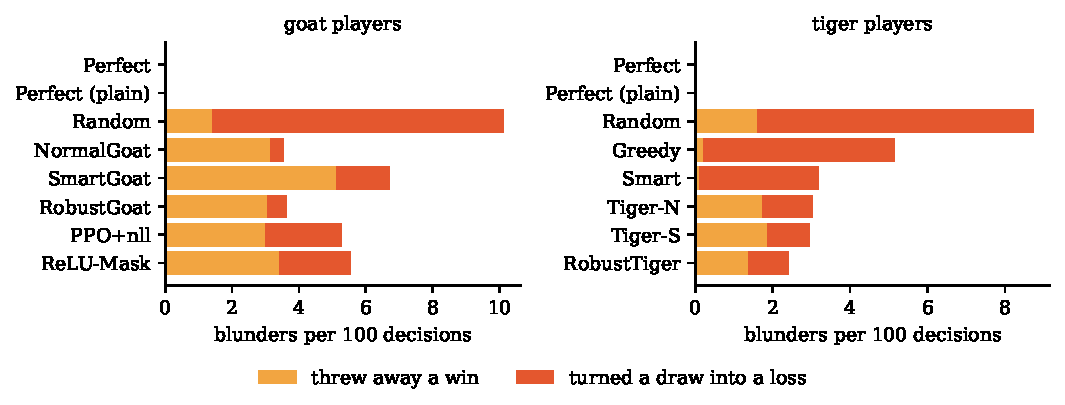
\includegraphics[width=\linewidth]{figures/blunders.pdf}
\caption{Blunders per 100 decisions, by kind, over all round-robin games of each player.}\label{fig:blunders}
\end{figure}

\subsection{Models against models}\label{sec:cmp-models}

Two deterministic models produce a single game, which says little. To get a distribution, the first four
plies are drawn uniformly from the moves that keep the game a draw; the models then play on. Those four
plies are not scored. Every game therefore starts from a different balanced position.

\begin{table}[H]
\centering\footnotesize
\caption{Goat models against tiger models from 200 balanced random openings, in percent. The last two
columns are blunders per 100 decisions of each side.}\label{tab:openings}
\begin{tabular}{@{}ll rrr r rr@{}}
\toprule
goats & tigers & goat wins & draws & tiger wins & plies & goat blunders & tiger blunders \\
\midrule
\tabin{generated/tab_openings}
\bottomrule
\end{tabular}
\end{table}

\subsection{The effect of the capture correction}\label{sec:cmp-fix}

The win rates of Section~\ref{old:9} were measured before the capture rule was corrected
(Section~\ref{sec:rulefix}); the round robin uses the corrected rule. To separate the two, the goat models
were replayed against the scripted tigers under both rules, 1{,}000 games each. Under the old rule a tiger
jumping from \code{d1} over \code{c1} to \code{b1} removes the goat on \code{b0} if there is one and otherwise
none.

\begin{table}[H]
\centering\footnotesize
\caption{Goat win rate under the old and the corrected capture rule (1{,}000 games per cell; standard error
at most 0.016). ``Study'' repeats the value of Sections \ref{old:9.1} and \ref{old:9.4}, measured in \code{TnGEnv}
before the correction. $\Delta$ is corrected minus old, in percentage points.}\label{tab:capturefix}
\begin{tabular}{@{}l rrrr rrrr@{}}
\toprule
 & \multicolumn{4}{c}{against Greedy} & \multicolumn{4}{c}{against Smart} \\
\cmidrule(lr){2-5}\cmidrule(l){6-9}
goats & study & old rule & corrected & $\Delta$ & study & old rule & corrected & $\Delta$ \\
\midrule
\tabin{generated/tab_capturefix}
\bottomrule
\end{tabular}
\end{table}

The ``old rule'' columns reproduce the study's values within sampling error, which confirms that the game
loop used here plays the same game as \code{TnGEnv} and that the difference in the other columns is the rule.

\subsection{Analysis}\label{sec:cmp-analysis}

\paragraph{1. Nobody beats the perfect player, and perfect against perfect is a draw.} All 800 games between
the two perfect players were drawn, 798 of them at the 200-ply limit and 2 by the repeat rule. In 5{,}600 games against other players a perfect player
never lost (Table~\ref{tab:roundrobin}, first two rows and columns). This is the solved value of the game seen
in play.

\paragraph{2. The goat models can all be beaten, some almost always.} Against the trap-seeking perfect tiger
the goats lose 11.5\% (NormalGoat), 29.5\% (RobustGoat), 83.5\% (SmartGoat), 84.0\% (ReLU-Mask) and 98.0\%
(PPO+nll) of their games (Table~\ref{tab:vsperfect}). A single $\D{\to}\Lo$ move decides each of these games: the
mean number of such blunders per game equals the loss rate, because the perfect tiger converts every one.
The first blunder comes late, on average between ply 43 and ply 91, well after the opening.

\paragraph{3. Strength against the training opponent and soundness are different things.} PPO+nll is the
strongest goat against the Smart tiger (96\% wins) and the easiest for a perfect tiger to beat (98\% losses).
NormalGoat wins only 2\% against Smart but holds a perfect tiger to a draw in 88.5\% of games. This is the
best-response effect of Section~\ref{sec:fp-br}: each model is tuned to the mistakes of its opponent and has
never been punished for its own. The longest-trained models (100M and 60M steps) are the hardest to exploit,
with SmartGoat the exception.

\paragraph{4. The tiger models fall into traps every time.} Against the trap-seeking perfect goat, all three
tiger models lose 200 games out of 200, in about 30 plies: they are immobilized as the placement phase ends.
The scripted Smart tiger survives 86.5\% of such games and even the Greedy tiger 34.5\%. Yet by average move
quality the tiger models are the \emph{best} non-perfect tigers, with 2.4--3.0 blunders per 100 decisions
against 3.2 for Smart (Table~\ref{tab:quality}). Against the plain perfect goat, which does not look for traps,
they draw 86--92\% of games. Average blunder rate measures typical play; exploitability measures the worst
case. A deterministic player with a few fixed weak spots can look good on the first and be lost on the second,
because a deterministic opponent that finds the weak spot finds it in every game.

\paragraph{5. A perfect player is not the best exploiter.} The plain perfect goat wins 17.5\% of its games
against Greedy and 1.5\% against Smart. NormalGoat wins 75\% against Greedy; PPO+nll wins 96\% against Smart.
Perfect play guarantees the value of the game, a draw, and nothing more: among moves that keep the draw it
has no reason to prefer the one the opponent is most likely to answer badly. Adding a one-ply preference
for traps raises the perfect goat to 65.5\% against Greedy, 13.5\% against Smart, 99.5\% against Random and 100\% against
the tiger models, still below the specialists against their own training opponent. The models earn their
wins by steering play into positions where that opponent errs: NormalGoat takes 46\% of its decisions in
positions that are already won for it.

\paragraph{6. Winning a won game is the hard part for some models.} Once a forced win is on the board, the
goat models convert it in 35\% (SmartGoat) to 90\% (ReLU-Mask) of games; the Random goat never does
(Table~\ref{tab:quality}). SmartGoat gives the win away in 30.7\% of its decisions in won positions, against
6.8--12.1\% for the other models. The tiger models give away 36--42\%, but for a tiger one wasted move in a
won position is often harmless, and they still convert all but one of the games in which they held a win.

\paragraph{7. Between models, the tigers come out ahead.} In the nine deterministic pairings of shipped models
the tigers win seven and draw two. From balanced random openings (Table~\ref{tab:openings}) the tigers win
between 19\% and 89\% of games and the goats at most 17.5\% (NormalGoat against RobustTiger). Blunder rates
are higher here than against scripted opponents, 5--14 per 100 decisions for the goats and 4--11 for the
tigers. A random opening and an unfamiliar opponent take both sides off the positions they were trained on.

\paragraph{8. The capture correction cost the models that leaned on the old rule.}
Table~\ref{tab:capturefix}: RobustGoat drops by 19 points against Greedy and 21 against Smart, and SmartGoat by
8 against Smart. Under the old rule a goat on \code{c1} could not be captured from \code{d1}, and these models
had learned to rely on it. NormalGoat and the two 10M-step models are unaffected (within one standard
error), although they too were trained under the old rule. All win rates in Section~\ref{old:9} should be
read with this in mind: they describe the game the models were trained on, not the corrected one.

\paragraph{9. Scale.} A uniformly random player makes 8.7 (tigers) to 10.1 (goats) blunders per 100
decisions. The trained models make 2.4--6.7. In drawn positions, where most decisions are made, the goat
models lose the draw in 0.8--3.3\% of decisions and the tiger models in 1.2--1.5\%, against 3.5\% for Smart
and 7.9\% for Greedy. The models have learned most of what keeps a position safe, and the remaining 1--3\% is
what a perfect opponent finds.

\paragraph{Limitations.}
\begin{itemize}
\item Each pairing has 200 games, so a percentage carries a standard error of up to 3.5 points.
\item Move quality in Table~\ref{tab:quality} pools a player's games against all opponents, which visit
  different positions. It ranks players loosely, not precisely.
\item Only games with the goats moving first were played. Models play deterministically.
\item The trap preference looks one ply ahead. A deeper search for the opponent's likely errors would
  exploit weak players more, at no risk.
\item One seed per training configuration, as in Section~\ref{old:9}.
\end{itemize}
